%  ========================================================================
%  Copyright (c) 1985-2014 The University of Washington
%
%  Licensed under the Apache License, Version 2.0 (the "License");
%  you may not use this file except in compliance with the License.
%  You may obtain a copy of the License at
%
%      http://www.apache.org/licenses/LICENSE-2.0
%
%  Unless required by applicable law or agreed to in writing, software
%  distributed under the License is distributed on an "AS IS" BASIS,
%  WITHOUT WARRANTIES OR CONDITIONS OF ANY KIND, either express or implied.
%  See the License for the specific language governing permissions and
%  limitations under the License.
%  ========================================================================
%

% Documentation for University of Washington thesis LaTeX document class
% by Jim Fox
% fox@washington.edu
%
%    Revised for version 2015/03/03 of uwthesis.cls
%
%    This document is contained in a single file ONLY because
%    I wanted to be able to distribute it easily.  A real thesis ought
%    to be contained on many files (e.g., one for each chapter, at least).
%
%    To help you identify the files and sections in this large file
%    I use the string '==========' to identify new files.
%
%    To help you ignore the unusual things I do with this sample document
%    I try to use the notation
%       
%    % --- sample stuff only -----
%    special stuff for my document, but you don't need it in your thesis
%    % --- end-of-sample-stuff ---


%    Printed in twoside style now that that's allowed
%
 
\documentclass [11pt, proquest] {uwthesis}[2015/03/03]
 
%
% The following line would print the thesis in a postscript font 

% \usepackage{natbib}
% \def\bibpreamble{\protect\addcontentsline{toc}{chapter}{Bibliography}}

\setcounter{tocdepth}{1}  % Print the chapter and sections to the toc
 

% ==========   Local defs and mods
%

% --- sample stuff only -----
% These format the sample code in this document

\usepackage{alltt}  % 
\newenvironment{demo}
  {\begin{alltt}\leftskip3em
     \def\\{\ttfamily\char`\\}%
     \def\{{\ttfamily\char`\{}%
     \def\}{\ttfamily\char`\}}}
  {\end{alltt}}
 
% metafont font.  If logo not available, use the second form
%
% \font\mffont=logosl10 scaled\magstep1
\let\mffont=\sf
% --- end-of-sample-stuff ---
 
\usepackage{color} 
 
\usepackage{graphicx}
\graphicspath{ {figures/} }


\begin{document}
 
% ==========   Preliminary pages
%
% ( revised 2012 for electronic submission )
%

\prelimpages
 
%
% ----- copyright and title pages
%
\Title{Smart Things and Cochlear Implants}
\Author{Tyler Ganter}
\Year{1985-2014}
\Program{UW Information Technology}

\Chair{Name of Chairperson}{Title of Chair}{Department of Chair}
\Signature{First committee member}
\Signature{Next committee member}
\Signature{etc}

% \copyrightpage

% \titlepage  

% --- sample stuff only -----
% unusual footnote not found in a real thesis
% You just use the \titlepage as commented out above

{\Degreetext{A dissertation%
  \footnote[2]{an egocentric imitation, actually}\\
  submitted in partial fulfillment of the\\ requirements for the degree of}
 \def\thefootnote{\fnsymbol{footnote}}
 \let\footnoterule\relax
 \titlepage
 }
\setcounter{footnote}{0}

% --- end-of-sample-stuff ---
 
%
% ----- signature and quoteslip are gone
%

%
% ----- abstract
%


\setcounter{page}{-1}
\abstract{%
This is my abstract
 
\begin{itemize}
\item here's an item
\footnote{here's a footnote}
\item item number 2
\end{itemize}
}
 
%
% ----- contents & etc.
%
\tableofcontents
\listoffigures
%\listoftables  % I have no tables
 
%
% ----- glossary 
%
\chapter*{Glossary}      % starred form omits the `chapter x'
\addcontentsline{toc}{chapter}{Glossary}
\thispagestyle{plain}
%
\begin{glossary}
\item[argument] replacement 
\item[back-up] a copy of a fi
 
\end{glossary}
 
%
% ----- acknowledgments
%
\acknowledgments{% \vskip2pc
  % {\narrower\noindent
  The author wishes to express sincere appreciation to
  University of Washington, where he has had the opportunity
  to work with the \TeX\ formatting system,
  and to the author of \TeX, Donald Knuth, {\it il miglior fabbro}.
  % \par}
}

%
% ----- dedication
%
\dedication{\begin{center}to my dear wife, Joanna\end{center}}

%
% end of the preliminary pages
 
 

%
% ==========      Text pages
%

\textpages
 
% ========== Chapter 1
 
\chapter{*Introduction}

this is the introduction

\section{*Overview}

\section{*Survey of Literature}

\section{*Contents of Thesis}

% ========== Chapter 2

\chapter{*Background}

\iffalse

\section{*PUT ELSEWHERE}	
	\subsection{types of audio}
	speech, music, harmonic, inharmonic, voiced, unvoiced
	tonal, non-tonal, consonant disonant..., transient, steady state

	\subsection{audio signal models}
	SUM [ A(t) * cos(wt + phi(t)) ]
	etc...
	TFS and envelope
	
	\subsection{cochlear implants}
	what is important?
		hearing for any general reason...safety, functionality
		speech recognition
	what is important and lacking?
		music appreciation
		tonal language
		SiN
		quality

\fi


\section{*Acoustic Hearing}

Before discussing how cochlear implants are able to restore hearing in people with profound hearing impairment, it is useful to talk about how acoustic hearing works in normal listeners.

\subsection{*Anatomy of the Ear}

tonotopic, critical bands, ...

\subsection{*speech}

\subsection{*pitch}

\subsection{*other characteristics of sound}

\section{*cochlear implants}
CI basics (CIS)
vague envelope concepts without math

"In spite of the fact that this analog signal itself preserves most of the original temporospectral in- formation, the signal transfers to the auditory nerve is handicapped by the limited maximal firing fre- quency of the auditory nerve in response to the electrical stimulation. High synchronization of nerve fibers and the neural refractory period only allow for frequency transmission up to 1 kHz via tempo- ral coding alone. For frequencies above 1 kHz, the spectral information cannot be sufficiently trans- ferred by temporal coding alone. Multichannel im- plants have been developed to make use of the tonotopic organization in the cochlea and thus transmit more spectral information to the auditory nerve." \cite{somek2006coding}


"The HiRes120 strategy, used in the Advanced Bionics implant, is the first commercial stimulating strategy that uses the virtual channel technique. Virtual channels are created by adjusting the current level ratio of two neighboring electrodes."

channel mapping
	why only 8 at a time?
	ACE vs CIS and benefits of each
	
	
	
	ACE uses place cues as the primary source of encoding a sound's characteristics.  To this day it is still unclear as to what implications this has.  This is due to a combination of factors including the subjective nature of pitch and absence of a ground truth baseline in many CI users.  For example, high-pass filtering a sound may cause it to sound brighter.  In contrast low-pass filtering would cause a warm quality.  As stimulus change electrodes a CI user could claim to experience changes in the high-low quality of pitch when really they are experiencing changes in the bright-warm quality of spectral distribution, or more likely an ambiguous combination of both.

There is general consensus that place cues are not sufficient for encoding pitch.  Alternatively, temporal cues encoded as time-domain carrier modulations have shown to be promising.

\section{*signal models}

A classic way of analyzing audio signals is the sum-of-products model.  In this model a signal is represented as a sum of narrowband signals $x_k[n]$ at distributed center frequencies.  Each of the narrowband components is modeled as a product of a slow-time-varying envelope $m_k[n]$ and a fast-time-varying carrier $c_k[n]$.

$$x[n] = \sum\limits_k x_k[n] = Re\bigg\{ \sum\limits_k m_k[n] c_k[n] \bigg\}$$

This model works especially well for harmonic signals, where each individual harmonic is represented by a narrowband component.  In the case of speech, one could think of the collection of carriers as the harmonic signal generated by the vocal tract, while the modulators together represent the resonant structure that distinguishes separate vowels. <--figure?!  Continue...

In this model information such as gender of talker, intonation or musical pitch would be dominantly characterized by the carriers.  The resonant information that distinguishes different vowels or the unique formant structure of a particular instrument would be encoded in the modulators.

The sum-of-products model is particularly convenient for CIs for a few different reasons. For starters, this model is naturally similar to the way our ears work. "mechanical fourier transform" [chimeara] The initial goal of CI researchers was to achieve speech recognition.  Given the limitations of CIs, encoding only the modulation information acts as a form of lossy data compression.

More reasons this model is good, musically?
Why is it good for CIs?

Provided the above motivation for sum-of-products signal modeling we come to the challenge of how exactly to decompose a signal.  There are many different ways of doing this but they broadly fall into one of two categories: incoherent methods and coherent methods.

\subsection{Incoherent Methods - Short Time Fourier Transform (STFT)}

With incoherent methods, an envelope is extracted independent of the carrier; no information about the carrier is taken into account prior to envelope extraction.

One such method is the short-time Fourier transform (STFT), which has two classic interpretations: a series of windowed Fourier transforms (each at a different time instant) or a collection of uniform bandpass filters (each at a different center frequency).  For our purposes we will be using the later.

An STFT bin at discrete time $n$ and discrete frequency $k$ is defined as:

$$X[n,k] = \sum\limits_{r=-\infty}^{\infty} x[r] w[r - n] e^{-j\frac{2\pi}{N}kr}, 0 \leq k < N$$

Defining a new variable $r' = r - n$ and defining our window such that  $w[n] = 0$ for $n < 0$ or $N \leq n$,

$$X[n,k] = \sum\limits_{r'=0}^{N-1} x[n + r'] w[r'] e^{-j\frac{2\pi}{N}k(n + r')}$$
$$= e^{-j\frac{2\pi}{N}kn} \sum\limits_{r'=0}^{N-1} x[n + r'] w[r'] e^{-j\frac{2\pi}{N}kr'}$$

Let $X[n,k]$ be represented in polar form as the following

$$X[n,k] = \vert X[n,k]\vert e^{j\angle X[n,k]}$$

If we assume that the window $w[n] \neq 0$ for $0 \leq n \leq N-1$ then we have the inverse

$$x[n + r'] = \frac{1}{Nw[r']}  \sum\limits_{k=0}^{N-1} X[n,k] e^{j\frac{2\pi}{N}k(n+r')}$$
$$= \frac{1}{Nw[r']}  \sum\limits_{k=0}^{N-1} \vert X[n,k]\vert e^{j(\frac{2\pi}{N}k(n+r') + \angle X[n,k])}$$
$$x[n] =\sum\limits_{k=0}^{N-1}  \frac{1}{Nw[0]}  \vert X[n,k]\vert e^{j(\frac{2\pi}{N}kn + \angle X[n,k])}$$

We can now clearly see our sum-of-products model

$$m_{k,STFT}[n] =  \frac{1}{Nw[0]}  \vert X[n,k]\vert$$
$$c_{k,STFT}[n] = e^{j(\frac{2\pi}{N}kn + \angle X[n,k])}$$

\subsection{*Incoherent Methods - Hilbert Transform}

Alternatively, a Hilbert transform uses the analytic signal to separate envelope from carrier.  We first acquire the bandpass signal

$$x_k[n] = x[n] * h_k[n]$$

Where $h_k$ is a bandpass filter and $k$ has arbitrary limits.  Then using the analytic signal

$$\widehat{x}_k[n] = x_k[n] + jH\{x_k[n]\}$$
$$m_{k,hilbert}[n] = \vert\widehat{x}_k[n]\vert$$
$$c_{k,hilbert}[n] = cos(\angle\widehat{x}_k[n])$$
OR
$$c_{k,hilbert}[n] = e^{j\angle\widehat{x}_k[n]}$$

Let us now compare this method to the STFT method.  Since "the Hilbert transform of a convolution is the convolution of the Hilbert transform on either factor" [wikipedia] we have 

$$\widehat{x}_k[n] = x_k[n] + jH\{x_k[n]\}$$
$$= x[n] * h_k[n] + jH\{x[n] * h_k[n]\}$$
$$= x[n] * h_k[n] + x[n] * jH\{h_k[n]\}$$
$$= x[n] * [h_k[n]+  jH\{h_k[n]\}]$$

Now let us define our filter specifically as

$$h_k[n] = \frac{1}{Nw[0]}w[-n]cos(\frac{2\pi}{N}kn)$$

If we assume the sidelobes of $w[n]$ roll-off sufficiently fast in relation to the center-frequency $\frac{2\pi k}{N}$, we may approximate

$$H\{h_i[n\}] \approx \frac{1}{Nw[0]}w[-n] H\{cos(\frac{2\pi}{N}in)\}$$
$$= \frac{1}{Nw[0]}w[-n]sin(\frac{2\pi}{N}in)$$

To verify the previous equation, consider the extremes:

1) $w[n] = 1$

2) $w[n] = \delta[n]$

TODO: verify this approximation claim

Plugging our explicit filter into the analytic signal equation (reference from above)

$$\widehat{x}_k[n] \approx x[n] * \frac{1}{Nw[0]}w[-n]e^{j\frac{2\pi}{N}in}$$
$$ =\frac{1}{Nw[0]}\sum\limits_{r=-\infty}^{\infty}x[n - r] w[-r] e^{j\frac{2\pi}{N}ir}$$
Let $r' = -r$

$$= \frac{1}{Nw[0]}\sum\limits_{r'=0}^{N-1} x[n + r'] w[r'] e^{-j\frac{2\pi}{N}kr'}$$


$$= \frac{1}{Nw[0]}\bigg[e^{-j\frac{2\pi}{N}kn} \sum\limits_{r'=0}^{N-1} x[n + r'] w[r'] e^{-j\frac{2\pi}{N}kr'}\bigg]e^{j\frac{2\pi}{N}kn}$$

$$ = \frac{1}{Nw[0]}X[n,i]e^{j\frac{2\pi}{N}kn}$$



What this tells us is that under the assumption of fast sidelobe rolloff we may define a filter bank of $N$ filters

$$h_k[n] = w[-n]cos(\frac{2\pi}{N}kn), 0 \leq k \leq N-1$$

such that

$$m_{k,hilbert}[n] \approx m_{k,STFT}[n]$$
$$c_{k,hilbert}[n] \approx Re\{c_{k,STFT}[n]\}$$

What this tells us is that the hilbert decomposition may be viewed as a superset of the STFT method that is not constrained to uniform bandwidth filters or linearly spaced filters.

\subsection{*Incoherent Methods - TODO}

Hilbert Envelope - where is this done in practice??
	sounds like hires120 does this

ACE - STFT as a bank of filters
pitch modulation in ACE


CIS - BPF -> rectification -> LPF   
	typically 200–400Hz cutoff frequency
	"Unlike ACE, all 16 frequency bands are then stimulated in sequence"


MAKE FREQ DOMAIN FIGS


\subsection{Coherent Methods - Spectral Center-of-Gravity}

Due to their LTI nature, incoherent methods fail to explicitly represent time varying characteristics like fundamental frequency or formant structure. \cite{wilson1993design}

One method is the spectral center-of-gravity (COG).  Similar to the previously described incoherent methods, spectral COG uses a fixed number of filters.  The key difference lies in the center frequency of each of these filters which adapt over time as a function of the spectral distribution within predefined band limits.

Spectral COG certainly has some advantages of better representation of the signal in comparison to incoherent methods, however it still doesn't escape the limitation of fixed and pre-determined band limits that each filter operates within.

\subsection{Coherent Methods - Harmonic}

To escape this, [Atlas and Others] proposed a harmonic method which uses knowledge of the structure of common audio signals to decompose the signal in a less arbitrary way.  The first step is to get a pitch estimate $F_0[n]$ of the signal.  We then define $k$ complex carriers where there is a hard limit as a function of Nyquist sampling rate, $k \leq  \lfloor \frac{F_s}{2F_0} \rfloor$

$$c_{k,harmonic}[n] = e^{jk\phi_0 [n]}$$

where 

% $$\phi_0[n] = \frac{2\pi}{F_s} \sum_{p=0}^{n} F_0[p]$$
$$\phi_0[n] = \phi_0[n - 1] + 2\pi \frac{F_0[n]}{F_s}$$
$$\phi_0[0] = 0$$
$$\phi_0[-n] = -\phi_0[n]$$

[modulation toolbox]

We define our bandpass signal as 

$$x_k[n] = x[n] * h_k[n]$$

and the analytic form

$$\widehat{x}_k[n] = x_k[n] + jH\{x_k[n]\}$$

where the key difference between this and the incoherent methods is that $h_k[n]$ is centered at $F_0$, that is, it changes adaptively as a function of $F_0$.

$$m_{k,harmonic}[n] = \widehat{x}_k[n] c_{k,harmonic}^*[n] $$

We may choose to design our filters such that

$$h_k[n] = \frac{1}{Nw[0]} w[-n] cos( k \phi_0[n])$$

where $w[n]$ is a lowpass filter and 
$$w[n] \neq 0, 0 \leq n < N$$
$$ = 0, else$$

In this case each bandpass filter has the same bandwidth and is simply shifted to a different center frequency as a function of $F_0$ and $k$.  This is a natural design since the spacing of harmonics is uniform in frequency.


$$m_{k,harmonic}[n] = \widehat{x}_k[n] e^{-jk \phi_0[n]}$$

Using eq (?.?) from [hilbert section]

$$m_{k,harmonic}[n] =  \Bigg[ x[n] * \Big[ h_k[n]+  jH\{h_k[n]\} \Big] \Bigg] e^{-jk \phi_0[n]}$$

$$=  \Bigg[ x[n] * \Big[ \frac{1}{Nw[0]} w[-n] cos( k \phi_0[-n]) +  jH\{\frac{1}{Nw[0]} w[-n] cos( k \phi_0[-n])\} \Big] \Bigg] e^{-jk \phi_0[n]}$$

Using eq (?.?) from [hilbert section]

$$\approx  \Bigg[ x[n] *  \frac{1}{Nw[0]} w[-n] \Big[cos( k \phi_0[-n]) +  jH\{cos( k \phi_0[-n])\} \Big] \Bigg] e^{-jk \phi_0[n]}$$

$$=  \Bigg[ x[n] *  \frac{1}{Nw[0]} w[-n] e^{jk \phi_0[-n]} \Bigg] e^{-jk \phi_0[n]}$$

$$= \sum_{r = -\infty}^\infty x[n - r] \frac{1}{Nw[0]}w[-r] e^{jk \phi_0[-r]} e^{-jk \phi_0[n]}$$

$$=  \frac{1}{Nw[0]} e^{-jk \phi_0[n]} \sum_{r = -\infty}^\infty x[n - r] w[-r] e^{jk \phi_0[-r]}$$

let $r' = -r$

$$= \frac{1}{Nw[0]} \bigg[ e^{-jk \phi_0[n]} \sum_{r' = 0}^{N-1} x[n + r'] w[r'] e^{jk \phi_0[-r']} \bigg]$$

as mentioned in (?.?) above, $\phi[-n] = -\phi[n]$

$$= \frac{1}{Nw[0]} \bigg[ e^{-jk \phi_0[n]} \sum_{r' = 0}^{N-1} x[n + r'] w[r'] e^{-jk \phi_0[r']} \bigg]$$

TODO: continue here


$$= \frac{1}{Nw[0]} X[n, k \phi_0[n] \frac{N}{2\pi n})$$

$$= \frac{1}{Nw[0]} X[n, k\lambda[n])$$

where we define $\lambda[n] = \phi_0[n] \frac{N}{2\pi n}$.  The "$)$" is a reminder that $k\lambda [n]$ is not restricted to integer values.  We can see the relationship to the STFT envelope as

$$\lambda[n] = 1 \Rightarrow \vert m_{k,harmonic}[n] \vert = m_{k,STFT}[n]$$

$$\lambda[n] = 1 \Rightarrow c_{k,harmonic}[n]e^{j \angle m_{k,harmonic}[n]} = c_{k,STFT}[n]$$



$$X[n,k] = e^{-j\frac{2\pi}{N}kn} \sum\limits_{r'=0}^{N-1} x[n + r'] w[r'] e^{-j\frac{2\pi}{N}kr'}$$


We can now see that the STFT envelope and magnitude of the harmonic envelope are related with two key differences:

1) $\lambda[n]$ is not necessarily an integer

2) $\lambda[n]$ is time-varying

It is important to note that in practice $\lambda[n]$ is not a continuous variable.  It is constrained by the quantization of the implemented pitch tracker.  That being said, there is no guarantee that this quantization will lead to integer values of $\lambda[n]$.

$$\lambda[n] = \lambda[n-1] + \frac{F_0[n]}{F_s}  \frac{N}{n}$$

So what exactly does $\lambda[n]$ represent?  TODO: 

1) STFT with zero-padding

2) need to consider $\lambda[n]$ changing faster than window hop factor (as in not constant over each STFT frame)

Moving on to the carriers, note that in the coherent harmonic method the phase information split into two components, one of which is part of the envelope.  We can think of this component as the fast variations unaccounted for by the smooth $F_0$ estimate as well as any drifting from $kF_0$ because the relationship is often not a perfect integer multiple or because the estimate of $F_0$ is off.



Talk about filter bandwidth, what is optimal? F0/2? F0/4?


With harmonic decomposition we are faced with a decision.  Our envelope is now complex, so if we need to use the envelope independent of carrier we must somehow convert it to a real signal.  The two natural options are two either take the real component or the magnitude.  Let me describe the advantages of each...


fft 0-padding as harmonic envelope computation!

		what does it mean to have a filter that changes
		between frames?  does it cause artifacts?


\subsection{Phase Vocoder}

phase vocoder or other?

\subsection{Modulator Bandwidth Tradeoff}

incorporating multiple harmonic components VS eliminating transient characteristics


LIT SEARCH!!!


% ========== Chapter 3

\chapter{CI DSP Strategies}


\section{A General Framework for CI Processing Strategies}

The main stages to processing in cochlear implants are visualized in Fig. ?? below.  While at every stage adjustments can be made, for the purpose of comparing DSP algorithms, all other stages will be assumed constant throughout this work unless otherwise specified.

In this section I will talk about the general differences between ACE, F0mod, HSSE

\begin{figure}[!ht]
  \centering
    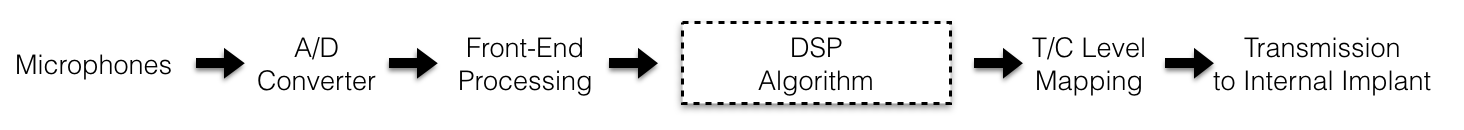
\includegraphics[width=1.0\textwidth]{CI_Signal_FlowTEMP}   
    \caption{Signal Flow in CI}
\end{figure}

In this document, the output of the DSP stage will be a strictly positive signal used to modulate a constant bipolar pulse train.

Returning to our discussion of sum-of-products models, each strictly positive signal will be composed of an envelope and carrier:

FIGURE
[DSP carrier * envelope] * pulse train = ~~~

In general we can think of the envelope as encoding the place information while the carrier encodes the temporal information

\subsection{ACE}

The simplest of the considered strategies is the Advanced Combination Encoder (ACE).  ACE has become a clinical standard for CI processing and is used in a vast number of users.  ACE is Cochlear Ltd's instance of the auditory community's generalized category of $N$-of-$M$ strategies.  In these strategies the magnitudes of the $L$ STFT envelopes are first extracted using the STFT extraction method.  These envelopes are then combined into $M$ channels corresponding uniquely to electrodes.  During each processing frame a subset $N$-of-$M$ channel envelopes is selected for stimulation on the internal implant.

$L$ - number of envelopes per frame

$M$ - number of electrode channels

$N$ - number of electrodes stimulated per frame

$$L \geq M \geq N$$

\begin{figure}[!ht]
  \centering
    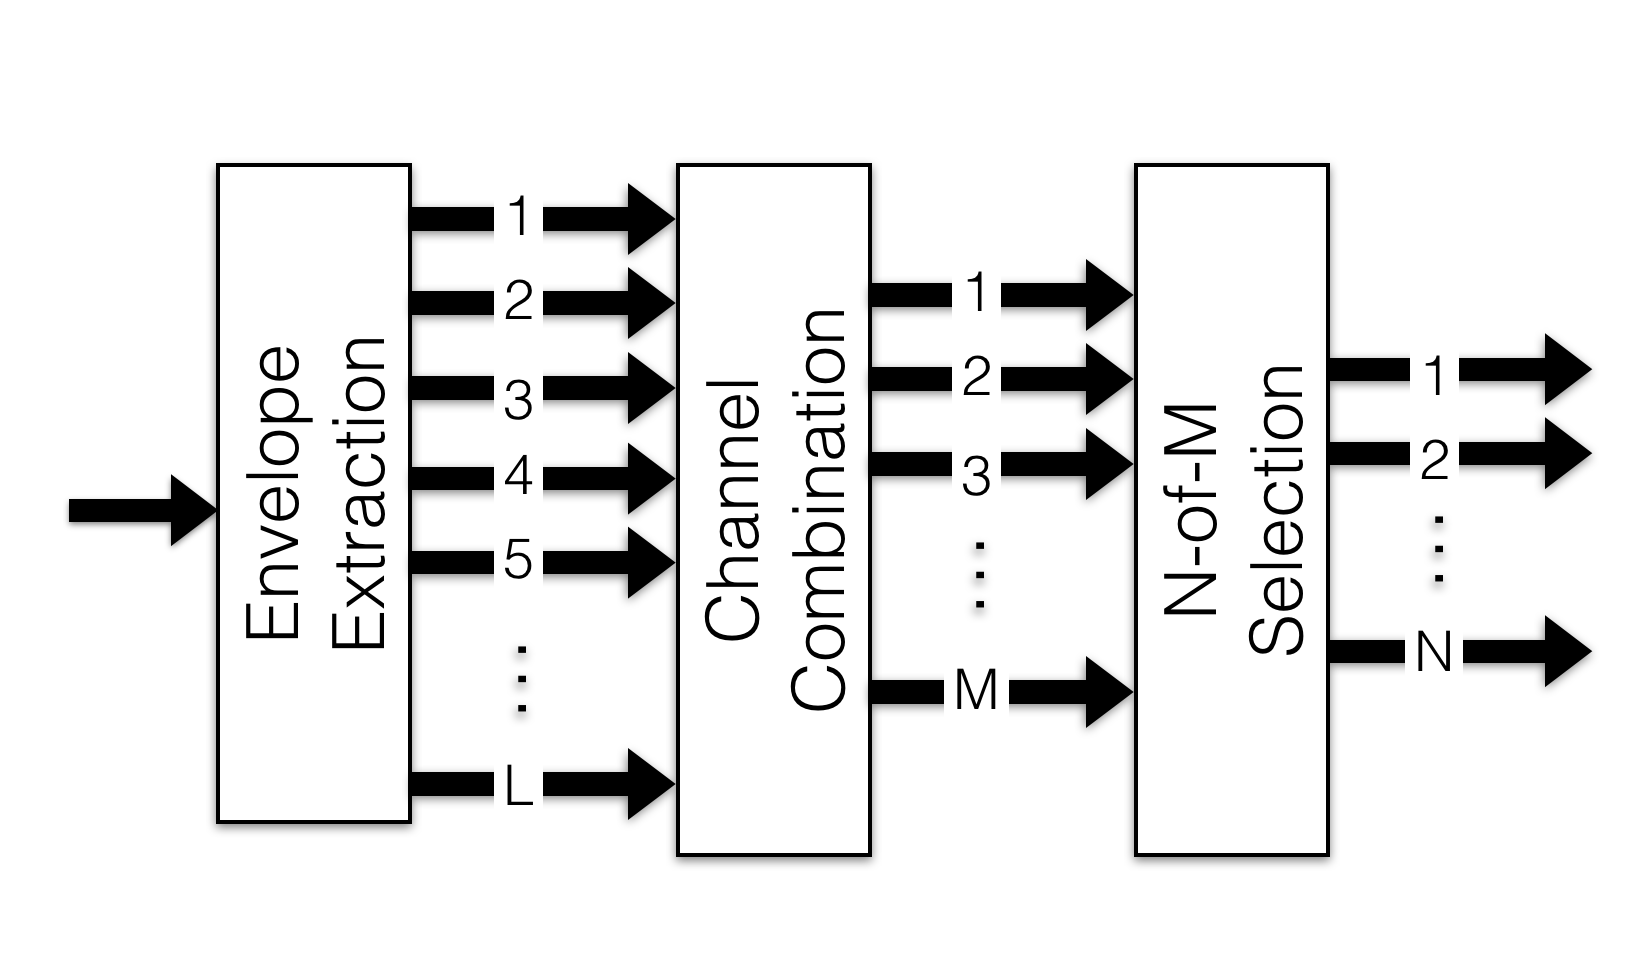
\includegraphics[width=0.5\textwidth]{ACE_flow_diagram_explicitTEMP}   
    \caption{ACE Flow Diagram}
\end{figure}

While ACE does a sufficient job for many CI users in speech recognition tasks, a large gap remains between NH and CI in pitch discrimination.  One important factor is that ACE uses place cues as the primary source of encoding a sound's characteristics.

ACE does, however, provide limited temporal modulations via beat frequencies.  This is a unique case of the filter bandwidth tradeoff in which wider bandwidth is desired to intentionally capture multiple harmonics in a band.  By doing this a beat-frequency will be induced at a rate of the difference between the two harmonic frequencies, i.e. $F_0$.  Typically these modulations are not full depth [ref?] and the depth is a function of filter rolloff, pitch and filter center frequency.  Modulations are usually limited to under ~250Hz [ref?]

The following figure is simply a condensed version of the previous flow diagram.  This condensed notation will be carried through to the other strategies analyzed.

\begin{figure}[!ht]
  \centering
    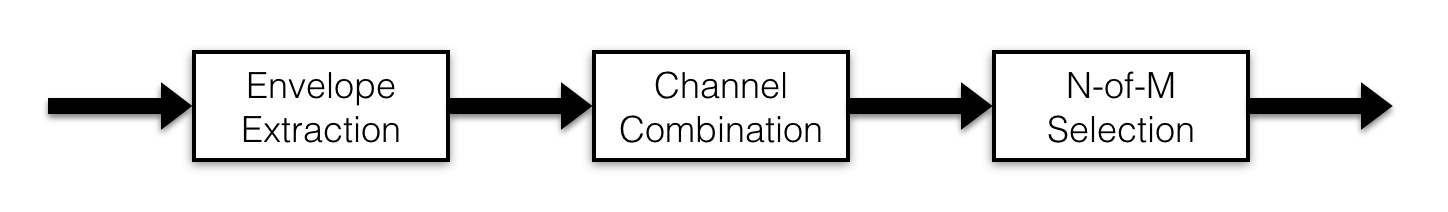
\includegraphics[width=1\textwidth]{ACE_flow_diagramTEMP}   
    \caption{condensed ACE Flow Diagram}
\end{figure}

\subsection{F0mod}

To get at the problem of pitch discrimination, (Laneau et al 2006) developed a new research strategy, F0mod.  F0mod provides the same processing as ACE with one important change, explicit carrier modulation.  It achieves this by adding a pitch estimator into the processing.

Once a fundamental frequency ($F_0$) is acquired, all output envelopes are modulated by a raised sinusoid at a rate of $F_0$.  

This raised sinusoid is constant modulation depth, (full dynamic range), and same across channels, (phase aligned).  *maybe show a figure?  The details of modulator type are discussed later in section ?.?.  The important point here is that modulations are applied at a rate of $F_0$ and full depth.

\begin{figure}[!ht]
  \centering
    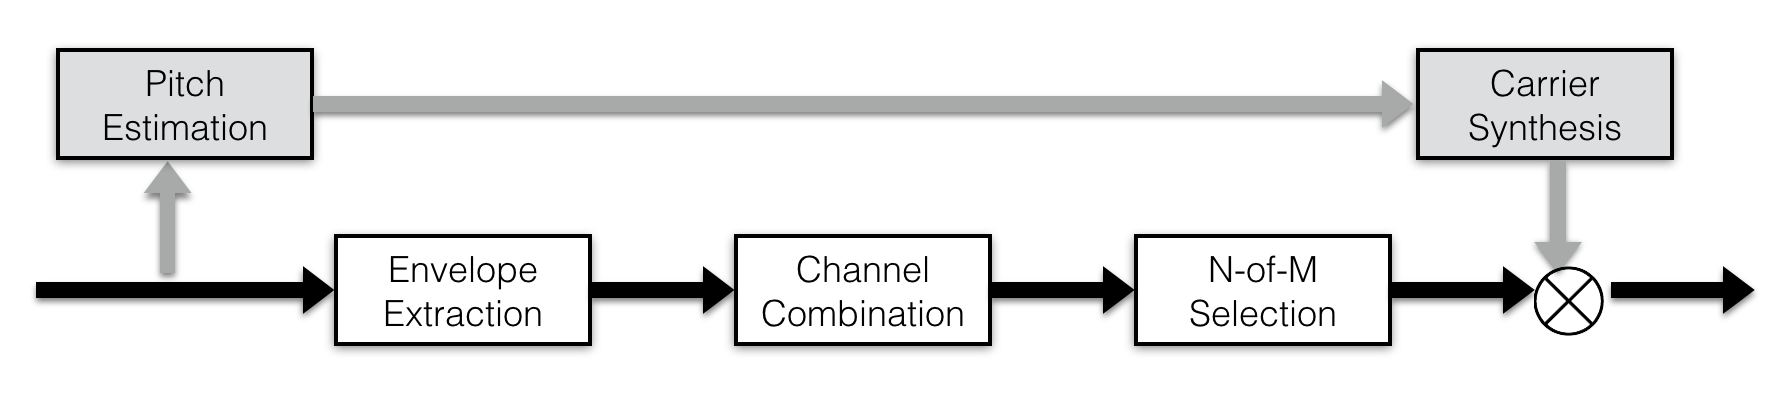
\includegraphics[width=1\textwidth]{F0mod_flow_diagramTEMP}   
    \caption{F0mod Flow Diagram}
\end{figure}

F0mod has shown promising results in acute tests for pitch discrimination.  It has also inspired other processing strategies such as eTone, which uses a more sophisticated harmonic sieve pitch estimator as well as soft decisions to overcome the problem of encoding both harmonic and inharmonic sounds as well as those that fall somewhere in between.

\subsection{HSSE}

Looking for a novel approach to improved pitch perception and more broadly music perception, (Li, Atlas, Nie) came up with Harmonic Single Sideband Encoder (HSSE).  HSSE uses coherent demodulation to extract $H$ harmonic envelopes.  These harmonic envelopes are then combined into channels based on the harmonic index and $F_0$.  Just as in F0mod a subset is selected for stimulation and then these envelopes are combined with carrier modulators.

$H$ - number of harmonic envelopes
$$H, M \geq N$$

\begin{figure}[!ht]
  \centering
    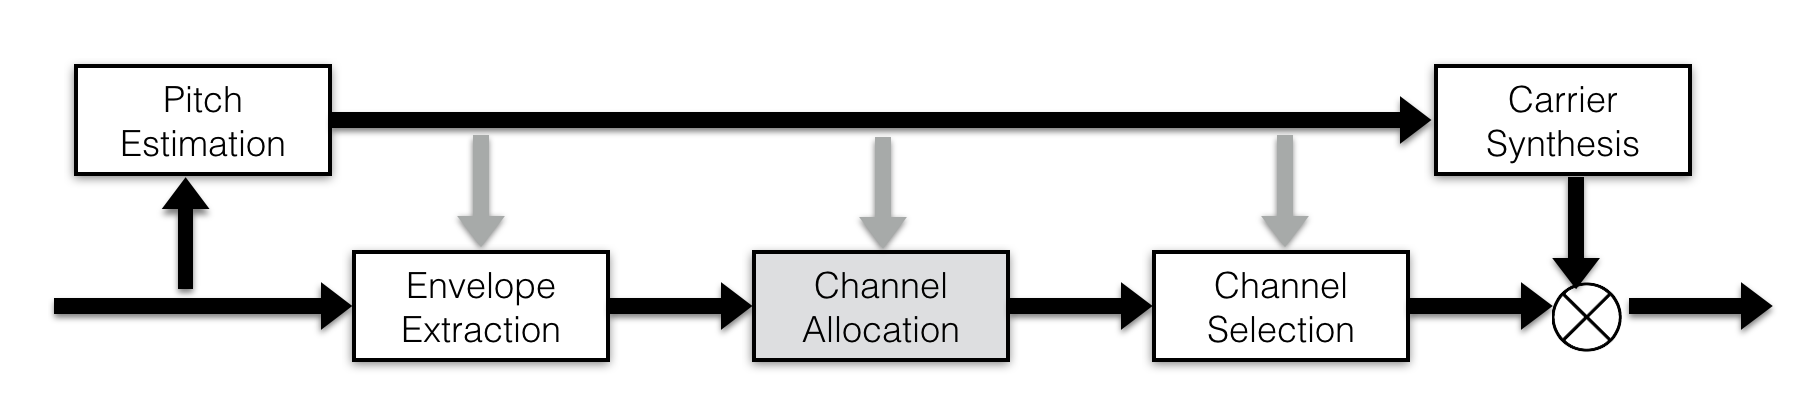
\includegraphics[width=1\textwidth]{HSSE_flow_diagramTEMP}   
    \caption{HSSE Flow Diagram}
\end{figure}

Sparing details which will soon be investigated deeper, the differences between F0mod and HSSE can be summarized quite simply;  Every stage of typical ACE processing is now done coherently using $F_0$ information.

It should be noted that it is not necessarily true that $H \geq M$.  In the case that no envelopes are allocated to a channel we may simply rule out that channel during the selection stage.

\subsection{*Other Strategies}

any hybrid considerations?  maybe hint at hsse ace hybrid

talk about unmentioned methods (AB, MedEl)

\subsection{Summary}

The considered strategies can be described by five general processing blocks: Pitch Estimation, Envelope Extraction, Channel Combination, Channel Selection and Carrier Synthesis.  We will now go into detail of each of these blocks, evaluating key considerations and differences.

\section{Pitch Estimation}

Fundamental Frequency Modulation is a key prospect in temporal encoding, shared by F0mod and HSSE, but not ACE.  There are various ways to estimate pitch with trade-offs for each.  We are going to assume the pitch estimator is the same when analyzing F0mod and HSSE.

talk about F0 estimator and alternatives...

	our (shared) technique
	e-tone? harmonic sieve, etc.
	latency, accuracy, octave errors and range restrictions,
	quantization

\section{*Envelope Extraction}

"tie the DSP theory into the pros and cons and limitations of CIs"

This is about Coherent vs Incoherent Envelopes and the details of each Incoherent method

how much detail are we going into?  Compare CIS, ACE, Hilbert.  Compare ACE128 to ACE512...

where do the matlab figs fall into play here?? (probably way later after math, etc)

Let's do more detailed figures highlighting the differences between F0mod/ACE and HSSE envelope techniques!

Fig: FFT -> Sum into Channels

Fig: Coherent Demod, maybe we need to talk about types of coherent envelopes first?

up until now we haven't needed to be explicit in what envelopes we are talking about, we now need to define these various terms:

incoherent vs coherent

harmonic vs hilbert (FFT bin)


\subsection{*Phase Preservation}

previous version of HSSE looked like: (preserve phase)

phase alignment has proven to be important in both HSSE and F0mod, but is that because we're screwing it up???

reduces the posibilites to just rectification, instead of various forms of modulation possible in CIs, (who cares though)

F0mod tries to separate magnitude and phase information.  HSSE recognizes this is a bad idea and keeps them together.

Math!

RESULTS:

 - do we need harmonic envelopes for this to matter?
 doesn't matter even when you use them

 - what are implications of downshift? what does it mean to apply phase to a different carrier? does this introduce a phase delay? what is it?
 Don't need to worry about it
 
 - hypothesis: phase needs to be scaled: phik(t) / k when signal is downshifted
 Totally true! explain this math
 
 - okay, magnitude is not really different, but still is sorta...phase is potentially very important though.  What happens to the phase with downshift, how does my hypothesis play into this, what if the pitch estimate is off by a little bit?  how well are the signals aligned when voiced or unvoiced?
 
used "shh" vs "saw" test.  at least when listening to the simulations, the processing essentially sounds like narrowband resonant filters.  The noise-like sounds are completely dominated by the filter bandwidth and the phase-information is not noticeable at all.

for high frequencies this works out because we would have needed to find a way to combine these non-phase-aligned envelopes

downshift frequencies are quantized to same as FFT (256 frequencies spaced 30Hz apart)
doesn't matter though, gain is same... (< -1.4dB dip)
NOT TRUE!!! Roll-off is not linear in dB, so since signal is not pure tone, components will roll off at faster or slower rates

\subsection{*Magnitude and Bin Alignment}

The human ear has much better resolution than the cochlear implant sound processor when decomposing a signal into frequency bands.  The artifacts of this can be clearly demonstrated by example.  In case1, the energy of the signal falls directly on the center frequency of an FFT bin.  In case2 the signal falls in between two bins.  In this case, neither bin represents the true energy of the signal.

HOWEVER:

Coherent is the Same (mathematically) as Hilbert, as ACE, as CIS except...for the downshift frequency.  This leads to a minimal (-1.6dB max) loss of gain for the desired frequency however it may lead to lower SNRs when desired frequency is further from center of filter and noise is closer to center of filter simultaneously.

show plots as well as math :D

\subsection{*Filter Design \& Bin Combination}

Woah...come back to CIS vs ACE etc for this!

\textbf{Bin Combo}

now that we have considered phase and magnitude, this component of HSSE can essentially be considered as a different combination of FFT bin magnitudes when compared to ACE.

as mentioned above hsse takes F0 into account and avoid bin alignment issues, however, inaccuracies in F0 estimate can lead to loosing high energy harmonics with narrowband filters.  likely need to just combine unless F0 estimator can be significantly improved

This is is where the critical band concepts come into play, would this mess up speech in noise goals? probably...but what can be done if we can't get a good pitch estimate?  filtering F0 could help this a bit but it introduces further delay

updating only 9 samples of downshift per frame rather than grabbing complete complex exponential could help however once the channels are combined it shouldn't matter

\textbf{Filter Design}

ACE currently uses modulations due to harmonic artifacts and low-order FFT.  This is horrible!  Let me explain why...it has nothing to do with the harmonic of interest and everything to do with the one harmonic below and one harmonic above the harmonic of interest.  Because this demodulation is done incoherently the modulation depths are not directly related to the harmonic of interest.  Furthermore, the cutoff is fixed and decided by parameters of the FFT and sampling rate which have nothing to do with the signal itself.  This makes the modulation even further unrelated to the signal.  (Could this also theoretically be a problem for F0mod?  Case: $F_0$ is very low and the harmonic lands right between two bins.  A small modulation could come about, ~probably not~)

An important detail to note is that of low-order-FFT induced modulations mentioned for ACE.  Laneau explicitly describes two different methods as ACE128 and ACE512 corresponding to different FFT orders.  F0mod uses ACE512 which keeps FFT bin modulations below roughly 60Hz in contrast to ACE128's 240Hz.  This sharper cutoff keeps envelope modulations out of the carrier frequency range, isolating this component and leaving the role of carrier modulation to the explicit modulator at $F_0$.

This segregation allows for easier relation to the modulation model of sounds.  Furthermore, F0mod is not prone to the modulation artifacts present in ACE128 and discussed in section 2.?.?

\subsection{*Unvoiced Signals}

I really hope!!!  This is well handled by two factors.

1) automatically choose high F0 when no good estimate exists.  This allows for higher frequencies (more important and more likely to be present in unvoiced) to be acquired.

2) If filters are adaptive bandwidth, the wide-bandwidth filters will preserve more high-frequency noise-like modulations.


 - Still no concrete solution for unvoiced signals, best answer so far is to have automatic high-F0 estimate during unvoiced sections (make it more stable than if bouncing between high and low)

\subsection{*Takeaway}

 - Phase Preservation doesn't matter (shh vs saw)
 
 - Magnitude also doesn't matter (-1.6dB)
 
 - HSSE may be viewed as a different way of combining FFT bin magnitudes.  I would argue that we do this using F0 for low frequencies, and fixed for high.  (critical bands!!!)

\section{*N-of-M Selection 1}

The key to HSSE here, is that we have isolated individual harmonics.  Harmonics are mapped to associated fixed channels due to the limitations of a fixed number of channels and fixed locations in the cochlea.  Because we have isolated individual harmonic envelopes there is no issue of signal energy falling in between channels.

\subsection{*Regularizer Heuristic}

Another bonus to HSSE is that we may add a simple heuristic to maintain channel mapping stability.  For example, if F0 has not varied significantly since the previous frame, we can allocate to the same channels to avoid unnecessary switching between channels induced by vibrato or inaccuracies in pitch estimation.

\subsection{*Multiple Harmonics Per Channel}
As far as having multiple harmonics in a single channel, there are a few solutions

1) Choose highest energy harmonic.

suffers from stability issues, what about gain?

2) Choose First

suffers from missing important harmonics in channel as well as misrepresenting unvoiced signals

3) Combine

How?  via sum of squares?

does a gain factor need to be applied to each channel?  how was this determined for ACE?

\subsection{*Takeaway}

Low Frequencies: stability heuristic keeps from jumping channels when on edge.

High Frequencies: not really relevant if critical bands are used

- gains?  maybe just use same as ACE since this should be pretty similar
 

\section{*N-of-M Selection 2}

Two general solutions

1) Adaptive (select loudest)

similar to ACE, we can choose the loudest channels.  This suffers from stability issues.  We can apply another heuristic to stabilize the decision based on consistency of signal energy and fundamental frequency

2) Fixed

stable, each option suffers from missing key harmonics to the signal

lowest channels will imply no high frequency energy, which could be bad for unvoiced signals

other relationships such as odd harmonics or prime numbered harmonics could miss harmonics critical to timbre perception.

What if we did F0mod with same channel selections as HSSE?  What would happen?

\subsection{*N-of-M Selection HSSE}

Various ideas have been proposed including $N$-largest and lowest-$N$.  Fixed Greenwood bands are determined offline, corresponding each electrode with a bandwidth.  The $N$ envelopes are then mapped to electrodes by finding the greenwood bands each harmonic falls within.


\subsection{*Takeaway}

 - Fixed VS MaximaSelect: this is still up in the air, Fixed is complicated by not necessarily having harmonic envelopes
 
 - for maxima select heuristics can be used to choose same if energy and F0 have not changed significantly
 


N-of-M, It is important to note that this is the same case for F0mod.  The carrier modulation is the same on each envelope and thus does not affect the selection process.
 
 


\section{*Carrier Synthesis}

talk about modulator types briefly

F0mod does raised

$$c_{ch}(t) = 0.5 + 0.5cos(2\pi F_0t)$$


We consider a few...cite paper

\section{*Alternative Real Method}

talk about HSSE real{} and why we aren't using it.

show math, flow diagrams and freq-domain figures

\section{*Conclusion}


% ========== Chapter 4

\chapter{*HHE}
come up with a better name!!!

MOTIVATION

\subsection{*HSSE vs F0mod Differences}

harmonics are resolved

 - how do we deal with should-be-unresolved harmonics?

channel combination

 - further considerations are needed

 - what does sum of squares mean? is it constant energy within the channel?  does it cause a gain or just average the channels?  look further into the gain component to ACE
 	it's just a <1 gain for multiple bins in one channel

 - can harmonics be combined? (higher harmonics) what does it mean to combine channel phase information?

channel selection

 - further considerations are needed

 - What if we did F0mod with same channel selections as HSSE?  What would happen?

\section{*HSSE vs F0mod More Differences}

recitified modulator (likely not too important)

also, pitch tilts

how can all of this be applied to soft decisions?

how can this all be done in real-time?

how are we accounting for non-linearities: AGC and sensitivity




\section{*Alternative Coherent Envelope Calculation using FFT bins}

This could all be achieved by zero padding

Math math math!

Incredibly frustrating...but do we even need this?  What about just choosing the nearest FFT bin.

Another consideration: 

\section{*Critical Bands}

talk about filter design in F0mod and HSSE and why non-uniform is better

\subsection{*HSSE vs ACE vs Human Ear}

In this subsection I will discuss the general differences in critical bandwidth:

1) how HSSE is too fine of a resolution
note: HSSE originaly had BW = F0/2, however hard to implement and still not like ear

2) how ACE is overall a poorer resolution

What about doing a hybrid?  This would further justify alternative HSUM in it's improved efficiency!  If summing together anyway, does it matter if harmonic envelopes are used or incoherent envelopes are used?

How about specifying the bandwidth at each electrode as apposed to the frequency boundaries

Bro, you need to look into Xing's method with multiple harmonics modulated at multiples of F0...
%curK in HSSE_all_harmonics_halfF0_8_dynamic_channel_Xing.m


\subsection{*Resolution Simulated by Adaptive Envelopes}

The human ear has orders of magnitude more filters than ACE, (roughly 1500/22 I think).

HSSE could simulate this higher resolution by choosing different filter center frequencies based on the input signal

\subsection{*Channel Selection Analysis}

ACE is like HSSE but for fixed FoI's.  We extract an envelope at the FoI and then transmit it to the associated electrode.

1) this goes back to what are the implications of ACE512 vs ACE128 vs coherent-envelope if we are summing anyway

2) can HSSE be reanalyzed in these terms to better justify wide-bandwidth filters for high frequencies?

Could channel selection concepts in HSSE be important?  Reflect on this in hindsight to recent discoveries.  By this I mean using memory to not switch channels excessively and other decisions that were brought into account.

\section{*Other Important Components}

Most everything so far has assumed the signal has an $F_0$, what if it doesn't?  What if it is well outside the boundaries of $F_0$?  What about polyphonic music?  What about SNRs below what is needed for accurate $F_0$ estimation.  What other flaws do these strategies have?  Mention eTone and other possible solutions, or why we justify not considering these problems.

\section{*Algorithm}

1) Filter Center Frequency
2) Filter BW
3) Effective Channel Information BW

\section{*Freedom details}

% ========== Chapter 5

\chapter{*Subject Tests}
initial results are...


	\subsection{*simulated real-time}
	
	\subsection{*mandarin tones pitch tilt}
	
	\subsection{*freedom processor}
		speech recognition...
		timbre recognition...
		other...


% ========== Chapter ??
 
\chapter{*Less Theoretical Stuff}

About this chappy

\section{*Engineering Decisions for Real-time}

1) 8 harmonics
this assumes we are dealing with musical instruments, speech is going to have characteristics well above the 8th harmonic.  A hope is that with inharmonic signals the estimate will automatically bounce to max($F_0$ estimate) which will thus hit the highest frequencies.  This also goes back to the hybrid idea


2) $F_0$ estimation downsampling details, ooOOooo, so impressive!

\section{*$F_0$ tilt, exageration}

mention the point that this was already done in Xing's paper, albeit $F_0/2$ without affine shift is more more likely to hit boundaries 

\section{*assembly implementation}

maybe show flow diagram or talk about 128-pt fft limitations



% ========== Chapter 6

\chapter{*Conclusion}

\section{*Summary}

\section{*Future Work}



%
% ==========   Bibliography
%
\nocite{*}   % include everything in the uwthesis.bib file
\bibliographystyle{plain}
\bibliography{ganter_thesis}
%
% ==========   Appendices
%
\appendix
\raggedbottom\sloppy
 
% ========== Appendix A
 
\chapter{Where to find the files}
 
The uwthesis class file, {\tt uwthesis.cls}, contains the parameter settings,
macro definitions, and other \TeX nical commands which
allow \LaTeX\ to format a thesis.  
The source to
the document you are reading, {\tt uwthesis.tex},
contains many formatting examples
which you may find useful.
The bibliography database, {\tt uwthesis.bib}, contains instructions
to BibTeX to create and format the bibliography.
You can find the latest of these files on:

\begin{itemize}
\item My page.
\begin{description}
\item[] \verb%http://staff.washington.edu/fox/tex/uwthesis.html%
\end{description}

\item CTAN
\begin{description}
\item[]  \verb%http://tug.ctan.org/tex-archive/macros/latex/contrib/uwthesis/%
\item[]  (not always as up-to-date as my site)
\end{description}

\end{itemize}

\vita{Jim Fox is a Software Engineer with UW Information Technology at the University of Washington.
His duties do not include maintaining this package.  That is rather
an avocation which he enjoys as time and circumstance allow.

He welcomes your comments to {\tt fox@uw.edu}.
}


\end{document}
